Actuators play a crucial role in the operation of robots by converting the rotational movement of a motor into linear motion, enabling the robot to perform various tasks. In the context of parallel robots, linear actuators are particularly important because they are responsible for the movements needed to control the robot's motion.

\begin{figure}[H]
    \centering
    \includegraphics[width=0.9\textwidth]{linear-motion-systems}
    \caption{Linear motion systems}
    \label{fig:linear-motion-systems}
\end{figure}

In parallel robots, linear actuators are used to manipulate the position and orientation of the end-effector. Traditional linear actuators include timing belts, rack and pinion systems, ball screws, and linear motors, as shown in Figure \ref{fig:linear-motion-systems}. However, these actuators often present challenges such as high cost, large size, and fixed or non-modifiable maximum stroke lengths.

The fixed or non-modifiable travel distance of conventional linear actuators is a major limitation, especially when the goal is to create a flexible platform capable of accommodating a wide range of rod-driven robot configurations. Flexibility is key to our platform, as it must adapt to various setups without requiring significant modifications.

Fortunately, parallel continuum robots open up a broader range of possibilities. Unlike traditional robots that move rigid elements, continuum robots use flexible elements like rods, which can be shortened or extended to achieve the desired motion. This concept is similar to the operation of 3D printer extruders (refer to Figure \ref{fig:extruder}).

\begin{figure}[H]
    \centering
    \begin{subfigure}[b]{0.4\textwidth}
        \includegraphics[width=\textwidth]{mk8-extruder}
        \caption{3D printer extruder}
        \label{fig:mk8-extruder}
    \end{subfigure}
    \begin{subfigure}[b]{0.4\textwidth}
        \includegraphics[width=\textwidth]{extruder-function}
        \caption{Functionality of extruder}
        \label{fig:extruder-function}
    \end{subfigure}
    \caption{3D printer extruder}
    \label{fig:extruder}
\end{figure}

3D printer extruders work by using a drive gear and a bearing to push and pull the filament towards the heater. For our application, we are not interested in the heating aspect but rather the mechanism that drives the filament. This mechanism can be adapted to move rods in our robot, as shown in Figure \ref{fig:extruder-wo-heater}.

\begin{figure}[H]
    \centering
    \includegraphics[width=0.5\textwidth]{creality-extruder}
    \caption{Extruder without heater}
    \label{fig:extruder-wo-heater}
\end{figure}

A custom design is necessary for several reasons. The filaments used in standard extruders are thicker than the rods suitable for our robots ($>1.75$ mm), as empirical experience suggests that rods thinner than 1.5 mm are ideal. Thicker rods require more force to bend, which these actuators are not designed to handle, making this thickness a practical upper limit for our application. Additionally, the width of the actuators must be considered, along with their weight and speed. Energy consumption is also a critical factor that must be taken into account.

\begin{figure}[H]
    \centering
    \includegraphics[width=0.55\textwidth]{actuators-arrange}
    \caption{Actuators arrange}
    \label{fig:actuators-arrange}
\end{figure}

Each rod requires its own actuator. Therefore, the actuators must fit within the stipulated diameter for the base of the arm. The top view of an actuator arrangement is shown in Figure \ref{fig:actuators-arrange}. For an arrangement of six actuators with width $W$ and distance to the center $c$, the relationship with the minimum base radius $R_{min}$ is shown in equations \ref{eq:w-rmin} and \ref{eq:r-rmin}. An original extruder has a width of $W=5.2$ cm with $c=0.7$ cm, which requires a minimum radius of $R_{min}=5.2$ cm according to equation \ref{eq:rmin}. This is larger than the model presented by \cite{wu2022}, and our aim is to design a smaller one. Therefore, we establish a minimum diameter of $R_{min}=3.5$ cm with a maximum $c=0.5$ cm, resulting in a maximum width of $W\approx3.5$ cm, according to equation \ref{eq:w-complete}.


\begin{align}
    \label{eq:r-rmin}
    r&=R_{min}-c\\
    \label{eq:w-rmin}
    W&=\frac{2}{\sqrt{3}}r\\
    \label{eq:w-complete}
    W&=\frac{2}{\sqrt{3}}(R_{min}-c)\\
    \label{eq:rmin}
    R_{min}&=\frac{\sqrt{3}}{2}W+c
\end{align}


\section{Motor}

The motor is the central component in actuators, and in extruders, stepper motors are commonly used. However, stepper motors were discarded for our application due to their size and speed limitations. Instead, we selected DC N20 geared motors, which are small and fast enough to meet our requirements. To control the number of revolutions accurately, a motor with an encoder is necessary (see Figure \ref{fig:n20-encoder}). The dimensions of the selected motor with encoder are specified in Figure \ref{fig:n20-encoder-dimensions}, and the specifications for the chosen variant are detailed in Table \ref{tab:motor-specs}.

\begin{figure}[H]
    \centering
    \includegraphics[width=0.45\textwidth]{n20-encoder}
    \caption{Gear motor N20 with encoder}
    \label{fig:n20-encoder}
\end{figure}

\begin{figure}[H]
    \centering
    \includegraphics[width=0.9\textwidth]{n20-encoder-dimensions}
    \caption{Dimensions of gear motor N20 with encoder}
    \label{fig:n20-encoder-dimensions}
\end{figure}


\begin{table}[H]
    \centering
    \caption{Gear motor specifications}
    \label{tab:motor-specs}
    \begin{tabular}{@{}ll@{}}
    \toprule
    Property                                     & Value                  \\
    \midrule
    Output shaft style                           & D-Shaft                \\
    Voltage range                                & $6-12$V                \\
    Speed (no load @ 6VDC)                       & $70$ rpm               \\
    Rated torque                                 & $0.65$ kg$\cdot$cm            \\
    Stall torque                                 & $4$ kg$\cdot$cm               \\
    Gear ratio                                   & 210:1                  \\
    Weight                                       & $15$g                  \\
    Encoder: cycles per revolution (motor shaft) & 3                      \\
    Encoder sensor type                          & Magnetic (Hall Effect) \\
    Hall response frequency                      & $100$ kHz              \\
    \bottomrule
    \end{tabular}
\end{table}

\section{First model}

A first concept of the linear actuator is shown in Figure \ref{fig:first-isometric-view}. This simple and straightforward model was designed to understand the basic concept of a linear actuator. The idea was to make it easy to manufacture using FDM (fused deposition modeling), specifically 3D printing. The width of this model is 46.06 mm (as shown in Figure \ref{fig:first-model-dimensions}), which exceeds the previously stipulated $~35$ mm. We found limitations when trying to reduce the actuator's width due to the diameters of the pulley, bearing, spring, and the length of the arm. Additionally, the bearing did not provide sufficient friction, necessitating improvements in this area. Enhancements were also needed for the motor grip and support to ensure ease of printing and overall functionality.

\begin{figure}[H]
    \centering
    \begin{subfigure}[b]{0.4\textwidth}
        \includegraphics[width=\textwidth]{first-isometric-view-frontal}
        \caption{Front isometric view}
        \label{fig:first-front-isometric-view}
    \end{subfigure}
    \begin{subfigure}[b]{0.4\textwidth}
        \includegraphics[width=\textwidth]{first-isometric-view-backwards}
        \caption{Back isometric view}
        \label{fig:first-back-isometric-view}
    \end{subfigure}
    \caption{First model isometric view}
    \label{fig:first-isometric-view}
\end{figure}

\begin{figure}[H]
    \centering
    \begin{subfigure}[b]{0.272\textwidth}
        \includegraphics[width=\textwidth]{first-model-frontal}
        \caption{Front view}
        \label{fig:first-model-frontal}
    \end{subfigure}
    \begin{subfigure}[b]{0.628\textwidth}
        \includegraphics[width=\textwidth]{first-model-top-view}
        \caption{Top view}
        \label{fig:first-model-top-view}
    \end{subfigure}
    \caption{First model dimensions}
    \label{fig:first-model-dimensions}
\end{figure}

\section{Final model}

After some iterations, the final model was developed, as shown in Figure \ref{fig:final-isometric-view}. The final design is more rounded to eliminate potential stress concentrators, and it is also more streamlined and material-efficient, incorporating holes in non-critical areas to reduce weight.

\begin{figure}[H]
    \centering
    \begin{subfigure}[b]{0.4\textwidth}
        \includegraphics[width=\textwidth]{final-isometric-view-front}
        \caption{Front isometric view}
        \label{fig:final-front-isometric-view}
    \end{subfigure}
    \begin{subfigure}[b]{0.4\textwidth}
        \includegraphics[width=\textwidth]{final-isometric-view-back}
        \caption{Back isometric view}
        \label{fig:final-back-isometric-view}
    \end{subfigure}
    \caption{Final model isometric view}
    \label{fig:final-isometric-view}
\end{figure}

Although the width remains the same, the arm, which previously collided with other actuators in an array, has been repositioned. It is now slightly shorter and rounded, as shown in Figure \ref{fig:final-model-dimensions}, allowing the arm to intrude into the space of another actuator without making contact at any point. This design maintains an array of 6 actuators within the established circle diameter of 7 cm.

\begin{figure}[H]
    \centering
    \begin{subfigure}[b]{0.316\textwidth}
        \includegraphics[width=\textwidth]{final-front}
        \caption{Front view}
        \label{fig:final-frontal}
    \end{subfigure}
    \begin{subfigure}[b]{0.584\textwidth}
        \includegraphics[width=\textwidth]{final-top}
        \caption{Top view}
        \label{fig:first-top}
    \end{subfigure}
    \caption{Final model dimensions}
    \label{fig:final-model-dimensions}
\end{figure}

The issue of friction was also addressed by adding an O-ring seal in a V-shaped bearing and creating a grooved pattern on the motor pulley. The space between the pulley was made narrower to enhance grip. Additionally, a pair of new components were designed to secure the motor, and an additional support was included over the arm and bearing for increased rigidity and safety. Critical parts such as the spring holder were reinforced, making them thicker to improve durability and performance.

Figure \ref{fig:final-actuator-explode} presents an exploded view of the final actuator, detailing each component with arrows and item numbers in balloons. The corresponding part names for the assembly are listed in Table \ref{tab:final-actuator-parts}, which also indicates the quantity and source of each part. The sources are categorized as 3D printed, commercial, or manufactured. Notably, the only "manufactured" part is the spring, which was custom-made.

\begin{figure}[H]
    \centering
    \includegraphics[width=0.8\textwidth]{actuator-final-explode}
    \caption{Actuator assembly exploded-view}
    \label{fig:final-actuator-explode}
\end{figure}
\begin{table}[H]
    \centering
    \caption{Actuator assembly parts list}
    \label{tab:final-actuator-parts}
    \begin{tabular}{llll}
    \toprule
    Item & Qty & Part Name / Description & Source \\
    \midrule
    1 & 1 & Base & 3D Printed \\
    2 & 1 & Motor GA12 N20 (must be with encoder) & Commercial \\
    3 & 2 & Motor Support & 3D Printed \\
    4 & 1 & Arm & 3D printed \\
    5 & 1 & V623ZZ Groove Pulley & Commercial \\
    6 & 1 & O-Ring - W2.62 x DI7.59 x DE2.83 & Commercial \\
    7 & 1 & Arm Support & 3D Printed \\
    8 & 2 & Phillips Countersunk Screw - DIN 965H M1.6x3 & Commercial \\
    9 & 1 & Pulley & 3D Printed \\
    10 & 3 & Binding Head Screw JIS B 1111 - M3x20 & Commercial \\
    11 & 1 & Binding Head Screw JIS B 1111 - M3x14 & Commercial \\
    12 & 1 & Binding Head Screw JIS B 1111 - M3x10 & Commercial \\
    13 & 1 & Binding Head Screw JIS B 1111 - M3x5 & Commercial \\
    14 & 3 & Hexagon Thin Nut DIN 439-2 - M3x0.5 & Commercial \\
    15 & 1 & Spring - D5.5x20mm & Manufactured \\
    \bottomrule
    \end{tabular}
\end{table}


\section{Specifications}

\begin{figure}[H]
    \centering
    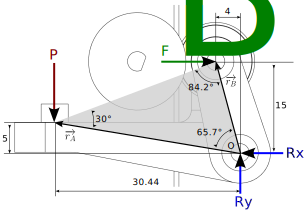
\includegraphics[width=0.8\textwidth]{forces-arm}
    \caption{Forces in actuator arm}
    \label{fig:forces-arm}
\end{figure}

The pressure or grip on the rod by the actuator is provided by the bearing and the actuator arm, whose static model is shown in Figure \ref{fig:forces-arm}. The sum of forces is found in Equation \ref{eq:sum-forces}, and the sum of moments at point $O$ is given in Equation \ref{eq:sum-momentums}. The force $P$ is exerted by the spring, as described by Equation \ref{eq:force-p}, where $k$ is the spring constant and $\Delta y$ is the compression. At the pin $O$, the components of the reaction force, $R_x$ and $R_y$, are present. From Equation \ref{eq:sum-momentums}, we can determine the reaction force $F_B$ at the bearing, as shown in Equation \ref{eq:force-fb}.

\begin{align}
    \label{eq:sum-forces}
    \sum \myvec{F}=0 \quad\therefore& \quad \myvec{P} + \myvec{R_y} + \myvec{F_B}+\myvec{R_x} = 0 \\
    \label{eq:sum-momentums}
    \sum \myvec{M_O}=0 \quad\therefore& \quad \myvec{r_A}\times\myvec{P} + \myvec{r_B}\times\myvec{F_B} = 0
\end{align}
\begin{equation}
    \label{eq:force-p}
    P=-k\Delta y
\end{equation}
\begin{equation}
    \label{eq:force-fb}
    F_B = \frac{r_{A,x}}{r_{B,y}}P = \frac{30.44}{15}P=-2.0293k\Delta y
\end{equation}

\begin{figure}[H]
    \centering
    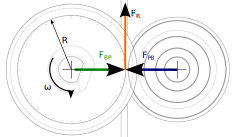
\includegraphics[width=0.7\textwidth]{friction-force}
    \caption{Friction force in rod}
    \label{fig:friction-force}
\end{figure}

From the force $F_B$, the friction force on the rod can be calculated, as shown in Figure \ref{fig:friction-force}, using Equation \ref{eq:force-fr}. However, these formulas were not applied in depth because static friction factors of the robot $\mu_s$ were measured instead. Geometric constraints were of greater importance. Therefore, the spring was selected by empirically testing those with the appropriate stiffness. The drive pulley, with radius $R$, rotates at speed $\omega$. Considering the motor's RPM, the actuator's speed specifications are provided in Table \ref{tab:actuator-specs}.

\begin{equation}
    \label{eq:force-fbp}
    F_{BP}=F_B
\end{equation}
\begin{equation}
    \label{eq:force-fr}
    F_{R}=\mu_{s}F_{BP}=-2.0293\mu_{s}k\Delta y
\end{equation}

\begin{table}[H]
    \centering
    \caption{Actuator specification}
    \label{tab:actuator-specs}
    \begin{tabular}{ll}
    \toprule
    Property & Value \\
    \midrule
    Pulley ratio ($R$) & $5.3$ mm \\
    Maximum angular velocity ($\omega_{max}$) & $7.3304$ rad/s \\
    Maximum linear velocity ($v_{max}$) & $38.85$ mm/s \\
    \bottomrule
    \end{tabular}
\end{table}